\documentclass{article}
\usepackage[utf8]{inputenc}
\usepackage{amsmath}
\usepackage{graphicx}
\usepackage{hyperref}
\usepackage{tikz}
\usepackage[a4paper,margin=1in,footskip=0.25in]{geometry}

\title{\textbf{Hypothetical Interventions on Sleep Stage Composition and Cognition and Brain Health} \protect\\ Analyis Plan}
\author{Lachlan Cribb \hspace{0.25cm} Beaudan Brown \and \\Stephanie Yiallourou \hspace{0.25cm} Matthew Pas\'e}
\date{\today}
\setlength{\parskip}{0.75em}
\begin{document}

\maketitle

\section{Introduction}
Insufficient slow wave sleep (SWS) has been associated with increased risk of dementia \cite{himali_association_2023}. SWS is thought to be important for glymphatic clearance of amyloid-$\beta$ and tau, the two hallmark features of Alzheimer's disease dementia. Restoring SWS may therefore reflect a potential intervention target to reduce risk of dementia. Similarly, an excessive proportion of time spent in light sleep (N1) has been associated with cognitive decline in older people \cite{song_relationships_2015}. A difficulty in interpreting these results, however, is the compositional nature of behavioural states. That is, time spent in each stage/state (N1, N2, N3, REM and wake) represents a compositional component of a 24 hour day. Therefore, if there is an increase in SWS, for example, then this time must come at the expense of another state (N1, N2, REM or wake). It may well be that the effect of increasing time in SWS depends on which other state(s) that time comes at the expense of.

Most, if not all, previous studies have utilised traditional regression tools, focusing on sleep stages in isolation. These methods assume that stages/states are independent of the other and unconstrained in time, which they are not (if one time use state increases another has to decrease). Thus, it is important to consider the co-dependent nature of time spent in behavioural states to determine the true effects of each state on CVD and dementia risk. To do this, we can apply the compositional data analysis (CoDA) approach, which treats states as inter-related within a constrained time period. This allows for estimating the association of reallocating time from one behavior/state to another on health outcomes whilst adjusting for the remaining state/behaviors. Thus, using this approach we can determine the benefits of increasing SWS at the expense of REM, for example, on cognitive and brain health as well as estimate an ideal composition (i.e., the ideal time spent in each state) of behavioural states for each outcome.

\section{Aims}
\begin{enumerate}
    \item To investigate the effect of increasing and decreasing time spent in each state (N1, N2, N3, or REM) when that time is coming at the expense or gain of time spent in different combinations of the other states (isotemporal substitutions).
    \item To find the "ideal" composition of states with respect to cognitive function and MRI volumetric outcomes. I.e., the absolute quantities of time spent in each state which is associated with the best cognitive performance and MRI volumetric outcomes.
\end{enumerate}

\section{Methods}

\subsection{Population}

Data are obtained from the Framingham Offspring Study (FOS) and the Sleep Heart Health Study (SHHS). SHHS is a multi-centre prospective cohort study designed to examine the cardiovascular outcomes of sleep-disordered breathing in middle-aged and older adults. Participants were recruited from multiple parent cohorts, including FOS, the Atherosclerosis Risk in Communities (ARIC) cohort, and the Cardiovascular Health Study (CHS). For this study, we used SHHS data provided by participants from the FOS study.

For SHHS, a sample of participants who met the inclusion criteria (see below) was invited to participate in the baseline SHHS examination (SHHS-1), which included a polysomnogram. A total of 997 individuals from the FOS study were enrolled between 1995 and 1998. A second polysomnogram (SHHS-2) was performed between 2001 and 2003 in 638 SOF participants.

For this study, we will use SHHS data from the Framingham Offspring Cohort, ARIC cohort, and CHS, all of which provide data on dementia events and cognition over follow-up.

\subsubsection{Eligibility criteria}

The following are the eligibility criteria for participation in SHHS:

\begin{itemize}
    \item Aged 40 or older
    \item No history of treatment for sleep apnea
    \item no Tracheostomy
    \item No current home oxygen therapy
\end{itemize}

\noindent For this study, we will additionally require that participants have SHHS-1 data available and apply the following exclusion criteria:

\begin{itemize}
    \item Dementia or other significant neurological disease prior to SHHS-2
    \item Mild cognitive impairment prior to SHHS-2
    \item Significant cardiovascular disease prior to SHHS-2
\end{itemize}

\subsection{Exposures}

Our variables of interest are the time spent in each state (wake, SWS, N1, N2, REM) at SHHS-2, obtained from overnight polysomnography. We use SHHS-2, rather than SHHS-1, for our exposure variables because it allows us to statistically adjust for SHHS-1. This ensures that the SHHS-2 sleep composition is approximately an "incident" exposure, thereby reducing confounding and selection bias related to past sleep behaviours.

\subsection{Confounders}

The presumed structure of confounding is displayed in the directed acyclic graph in Figure \ref{fig:dag}. $A$ represents sleep stage composition at SHHS-2, which is the exposure. $L_0$ represents confounders measured at or near SHHS-1 and includes age, sex, education, race, MMSE score, body mass index (BMI), waist circumference, physical activity (from the PAI), hypertension, CVD, diabetes, smoking status, APOE $\epsilon$ 4 positivity, medication (sedative, sleeping pill, antidepressant), apnea hypopnea index, MRI intracranial volume (for MRI outcomes only), and appropriately transformed SHHS1 Sleep macro-architecture measures: time in N1, N2, N3, REM, time awake, wake after sleep onset (WASO), sleep maintenance efficiency, and apnea hypopnea index. and . $L_t$ represents covariates variables measured at time $t$. $U$ is a vector of unmeasured variables (e.g., genetics) which is a common cause of sleep stage composition, covariates $L$, death $D$, and the outcome $Y$.

\begin{figure}[h]
    \centering
    \usetikzlibrary{positioning}
    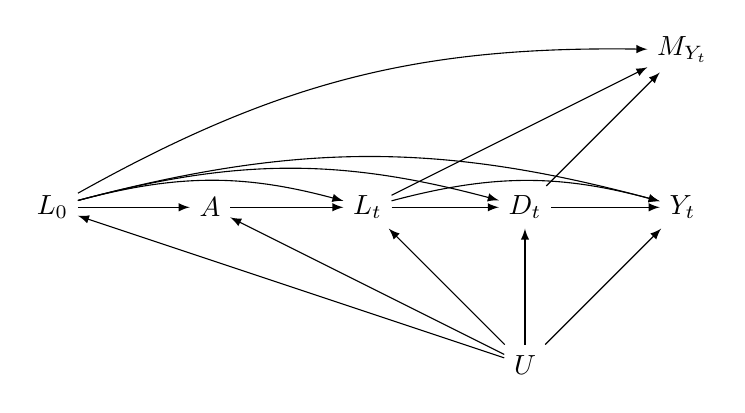
\begin{tikzpicture}[every node/.append style={draw, minimum size=0.5cm}]
        \node [draw=none] (L) at (0,0) {$L_{0}$};
        \node [draw=none] (A) at (2,0) {$A$};
        \node [draw=none] (Lt) at (4,0) {$L_{t}$};
        \node [draw=none] (Dt) at (6,0) {$D_{t}$};
        \node [draw=none] (Yt) at (8,0) {$Y_{t}$};
        \node [draw=none] (MYt) at (8,2) {$M_{Y_t}$};
        \node [draw=none] (U) at (6,-2) {$U$};

        \draw [-latex] (L) edge (A);
        \draw [-latex] (L) edge [bend left=15] (Lt);
        \draw [-latex] (L) edge [bend left=15](Dt);
        \draw [-latex] (L) edge [bend left=15] (Yt);
        \draw [-latex] (L) edge [bend left=15] (MYt);
        \draw [-latex] (Lt) edge (Dt);
        \draw [-latex] (Lt) edge [bend left=15] (Yt);
        \draw [-latex] (Lt) edge (MYt);
        \draw [-latex] (A) edge (Lt);
        \draw [-latex] (U) edge (Dt);
        \draw [-latex] (U) edge (A);
        \draw [-latex] (U) edge (Yt);
        \draw [-latex] (U) edge (L);
        \draw [-latex] (U) edge (Lt);
        \draw [-latex] (Dt) edge (MYt);
        \draw [-latex] (Dt) edge (Yt);
    \end{tikzpicture}
    \caption{Directed acyclic graph}
    \label{fig:dag}
\end{figure}

The directed acyclic graph encodes the following assumptions:
- Outcome data missing at random, conditional on covariates

\subsection{Follow-up}
Follow-up commences at the time of SHHS-2 (the time of exposure measurement).

\subsection{Outcomes}
\begin{itemize}
    \item Incident dementia
    \item Global cognitive factor score
    \item Domain specific cognitive factor scores
    \item MRI volumetric outcomes (total brain volume, grey matter volume, white matter volume, hippocampal volume, white matter hyperintensities)
\end{itemize}

\subsection{Statistical analysis}

\subsubsection{Isotemporal substitutions}

Prior to fitting regression models, compositional variables (time in N1, N2, N3, REM, WASO, and other wake) will be transformed from the simplex to the unconstrained Real space using an isometric log-ratio transformation (ILR). These ILR coordinates will be used in subsequent steps.

To estimate the effect of increasing or decreasing time in each sleep state, with that time coming at the expense or gain of each other state (e.g., an increase in SWS at the expense of REM), we will use the following algorithm:

\begin{itemize}
    \item Estimate the parameters of a multivariate normal to describe the joint distribution of the SHHS2 ILR coordinates, conditional on the covariates.
    \item Fit a regression model for the outcome, including SHHS2 ILR coordinates and covariates as predictors. This is a linear regression model for continuous outcomes and a pooled logistic model for survival outcomes. Models include restricted cubic splines for numeric variables and exposure-covariate and covariate-covariate product terms.
    \item Compute, based on the fitted model, the mean outcome under "no intervention" (i.e., the mean outcome when the SHHS2 sleep stage composition is left at its observed level) by g-computation.
\end{itemize}

For each isotemporal substitution of interest (e.g., adding 10 minutes of N3 at the expense of REM):

\begin{itemize}
    \item Apply the isotemporal substitution to the observed ILR coordinates. This substitution is **only** applied for those participants for whom the probability density of the shifted distribution, according to the multivariate normal fitted above, is greater than a threshold.
    \item Estimate the mean outcome under the composition resulting from this isotemporal substitution by g-computation.
    \item Calculate a mean difference (for continuous outcomes) or risk difference/ratio (for survival outcomes) between the no intervention and isotemporal substitution compositions.
\end{itemize}

\subsubsection{Ideal and worst composition}

To estimate the ideal and worst composition, i.e., the absolute time spent in each sleep stage associated with the best and worst outcome, respectively, we will use the following method:

\section{References}
\bibliographystyle{plain}
\bibliography{citations}

\end{document}
